\documentclass[tikz, border = 5pt]{standalone}

\begin{document}
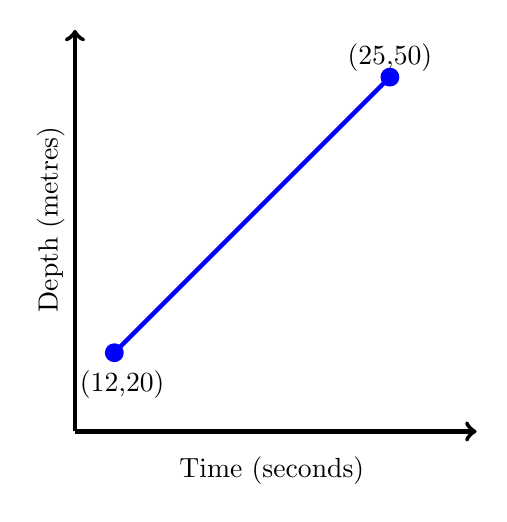
\begin{tikzpicture}
 
 % axis
  \draw[ultra thick, ->] (0, 0) -- (0, 5.1);
  \draw[ultra thick, ->] (0, 0) -- (5.1, 0);
\node[rotate=90] at (-0.5,2.5,-0.5) {Depth (metres)};
\node[] at (2.5,-0.5) {Time (seconds)};

  % grid
  %\draw[help lines, step = 0.5cm] (0, 0) grid (5, 5);

\draw[ultra thick, scale=0.5, domain=1:8,smooth,variable=\x, blue] plot ({\x},{1*\x+1});
\draw [draw=blue, fill=blue, thick] (.5,1) circle (3.0pt);
\draw [draw=blue, fill=blue, thick] (4,4.5) circle (3.0pt);
\node[] at (.6,.6) {(12,20)};
\node[] at (4,4.75) {(25,50)};
\end{tikzpicture}
\end{document}
